% =====================================================================
%  Extended Data for the Wuhan-Shanghai optical-clock comparison
%  (paper/rev2/extended_data.tex -- standalone document)
%
%  Companion document to main.tex. Every number is a macro generated by
%  tools/build_numbers.py; tables are generated artifacts under
%  generated/. Do not edit numbers by hand.
%
%  Compile:  pdflatex extended_data.tex && pdflatex extended_data.tex
% =====================================================================
\documentclass[11pt,a4paper]{article}

\usepackage[T1]{fontenc}
\usepackage[utf8]{inputenc}
\usepackage{amsmath}
\usepackage{amssymb}
\usepackage{graphicx}
\usepackage{booktabs}
\usepackage{geometry}
\usepackage[hidelinks]{hyperref}

\usepackage{siunitx}
\sisetup{detect-all,separate-uncertainty=true,group-digits=all,group-minimum-digits=4}

\geometry{margin=2.5cm}

% Generated by tools/build_numbers.py -- do not edit by hand.
% Provenance for every macro: generated/numbers_manifest.json.

\newcommand{\Rheadline}{1.207\thinspace507\thinspace039\thinspace343\thinspace337\thinspace720\thinspace1}
\newcommand{\RbayesFull}{1.2075070393433377201344585656369188179292550569336320493567391993015505600807042}
\newcommand{\RwlsFull}{1.2075070393433377201300363286261481205336963758023772463919635856100035202592917}
\newcommand{\RmpFull}{1.2075070393433377201300363286261481205336963758023772463919635856100035202592917}
\newcommand{\RwlsHead}{1.207\thinspace507\thinspace039\thinspace343\thinspace337\thinspace720\thinspace1}
\newcommand{\RmpHead}{1.207\thinspace507\thinspace039\thinspace343\thinspace337\thinspace720\thinspace1}
\newcommand{\RbayesHead}{1.207\thinspace507\thinspace039\thinspace343\thinspace337\thinspace720\thinspace1}
\newcommand{\RwlsHeadT}{1.207\thinspace507\thinspace039\thinspace343\thinspace337\thinspace720\thinspace130}
\newcommand{\RmpHeadT}{1.207\thinspace507\thinspace039\thinspace343\thinspace337\thinspace720\thinspace130}
\newcommand{\RbayesHeadT}{1.207\thinspace507\thinspace039\thinspace343\thinspace337\thinspace720\thinspace134}
\newcommand{\RwlsRawT}{1.207507039343337720130}
\newcommand{\RmpRawT}{1.207507039343337720130}
\newcommand{\RbayesRawT}{1.207507039343337720134}
\newcommand{\uStatE}{1.139}
\newcommand{\uStatShort}{1.14}
\newcommand{\uWlsE}{1.128}
\newcommand{\uMpE}{1.128}
\newcommand{\uBirgeE}{0.725}
\newcommand{\chiSq}{6.18}
\newcommand{\chiRed}{0.412}
\newcommand{\dofV}{15}
\newcommand{\pChi}{\ensuremath{9.8\times10^{-1}}}
\newcommand{\birgeRatio}{0.642}
\newcommand{\xiMpE}{0.00}
\newcommand{\xiBayesE}{0.14}
\newcommand{\muBayesE}{\ensuremath{-0.676}}
\newcommand{\sensRwlsHead}{1.207\thinspace507\thinspace039\thinspace343\thinspace337\thinspace720\thinspace4}
\newcommand{\sensChiRed}{0.51}
\newcommand{\dSegNineWls}{\ensuremath{+0.29\times10^{-18}}}
\newcommand{\tidalChiRaw}{0.41}
\newcommand{\tidalChiTheory}{0.57}
\newcommand{\tidalChiEmp}{0.54}
\newcommand{\tidalShiftEmpE}{0.85}
\newcommand{\tidalShiftAltE}{0.21}
\newcommand{\tidalChiAlt}{0.50}
\newcommand{\nSeg}{16}
\newcommand{\nSegAll}{17}
\newcommand{\nSamples}{986\thinspace416}
\newcommand{\nSamplesAll}{1\thinspace008\thinspace912}
\newcommand{\nHours}{274}
\newcommand{\nHoursAll}{280}
\newcommand{\nSegNine}{22496}
\newcommand{\nModelLimited}{5}
\newcommand{\modelLimitedGroups}{\ensuremath{2,\ 6,\ 7,\ 12,\ 16}}
\newcommand{\uSrE}{0.92}
\newcommand{\uYbE}{1.3}
\newcommand{\uLinkE}{0.1}
\newcommand{\uCombE}{0.1}
\newcommand{\uTidalE}{0.85}
\newcommand{\dWVal}{280.042}
\newcommand{\dWUnc}{0.085}
\newcommand{\dWAlt}{280.60}
\newcommand{\dWAltUnc}{2.558}
\newcommand{\refNistV}{1.207\thinspace507\thinspace039\thinspace343\thinspace337\thinspace723\thinspace0}
\newcommand{\refNistU}{37}
\newcommand{\refNistE}{3.7}
\newcommand{\refEuV}{1.207\thinspace507\thinspace039\thinspace343\thinspace337\thinspace718}
\newcommand{\refEuU}{32}
\newcommand{\refEuE}{3.2}
\newcommand{\fibreKm}{1\thinspace350}
\newcommand{\roundKm}{2\thinspace700}
\newcommand{\siteKm}{700}
\newcommand{\levelKm}{1\thinspace113}
\newcommand{\nDays}{58}
\newcommand{\nStages}{3}
\newcommand{\refSameCampusU}{\ensuremath{3.2\times10^{-18}}}
\newcommand{\refSameCampusKm}{3.6}
\newcommand{\refEuBestU}{\ensuremath{7.7\times10^{-18}}}
\newcommand{\refPtbTransportableU}{\ensuremath{4.3\times10^{-18}}}
\newcommand{\baconE}{\ensuremath{8\times10^{-18}}}
\newcommand{\nemitzU}{\ensuremath{5\times10^{-17}}}
\newcommand{\refVlbiKm}{9\thinspace000}
\newcommand{\refLisdatKm}{1\thinspace415}
\newcommand{\fRepMHz}{200}
\newcommand{\fFifteenTHz}{193.3992}
\newcommand{\deltaGV}{\ensuremath{-3.116\times10^{-15}}}
\newcommand{\uSubsystemBound}{\ensuremath{1\times10^{-19}}}
\newcommand{\levelMm}{0.255}
\newcommand{\refThreshold}{\ensuremath{5\times10^{-18}}}
\newcommand{\selfEvalBound}{\ensuremath{2\times10^{-18}}}
\newcommand{\refLisdatU}{\ensuremath{5\times10^{-17}}}
\newcommand{\euNClocks}{7}
\newcommand{\euNInstitutes}{4}
\newcommand{\lindvallNClocks}{10}
\newcommand{\lindvallNCountries}{6}
\newcommand{\lindvallNRatios}{38}
\newcommand{\schioppoKm}{\ensuremath{2\,220}}
\newcommand{\chenKm}{\ensuremath{2\,067}}
\newcommand{\claimDate}{October 2026}
\newcommand{\uStaticE}{0.946}
\newcommand{\uTotalE}{2.34}
\newcommand{\uTotalShort}{2.3}
\newcommand{\RheadlineUnc}{28}
\newcommand{\dVsNistE}{\ensuremath{-2.87\times10^{-18}}}
\newcommand{\dVsEuE}{\ensuremath{+2.13\times10^{-18}}}


\newcommand{\dff}{\Delta f/f}
\newcommand{\dW}{\Delta W}

\title{Extended Data: Intercity Yb/Sr optical clock comparison over
\fibreKm\,km fiber link at \uTotalShort$\times10^{-18}$}

\author{xxxxx}

\date{}

\begin{document}
\maketitle

\section{Extended Data}

\begin{table}[h]
  \centering
  \caption{Per-segment data of the 16 segments analyzed in this work.
  Ratio deviations $y_i = R_i/R_1 - 1$ are relative to the first
  segment, with $R_1 = \RsegOne$. $u(y_i)$ is the statistical
  uncertainty of the segment ratio;
  ``Fit'' is \emph{est.} for segments whose stability fit lies in the
  white-frequency-noise band and \emph{lim.} for model-limited fits.}
  \label{tab:segments}
  % Generated by tools/build_numbers.py -- do not edit by hand.
\begin{tabular}{rrrrl}
\toprule
Group & $n_{\rm valid}$ & $y_i$ ($10^{-18}$) & $u(y_i)$ ($10^{-18}$) & Fit \\
\midrule
1 & 68\,009 & +0.00 & 4.245 & est. \\
2 & 29\,481 & -3.36 & 3.017 & lim. \\
3 & 42\,891 & +2.00 & 5.880 & est. \\
4 & 64\,280 & -4.61 & 3.674 & est. \\
5 & 19\,532 & -3.38 & 15.250 & est. \\
6 & 52\,140 & -1.15 & 2.230 & lim. \\
7 & 39\,526 & +5.31 & 3.476 & lim. \\
8 & 43\,565 & +0.97 & 9.860 & est. \\
10 & 57\,938 & -0.76 & 5.003 & est. \\
11 & 35\,824 & +2.61 & 5.976 & est. \\
12 & 40\,346 & +0.73 & 4.843 & lim. \\
13 & 152\,994 & -3.09 & 4.019 & est. \\
14 & 68\,618 & +1.97 & 6.254 & est. \\
15 & 57\,649 & -0.25 & 4.028 & est. \\
16 & 147\,640 & -0.77 & 1.809 & lim. \\
17 & 65\,983 & -0.89 & 8.813 & est. \\
\bottomrule
\end{tabular}

\end{table}

\begin{table}[h]
  \centering
  \caption{Leave-one-out sensitivity of the ratio combination. Each
  row excludes one of the 16 segments and recomputes the combination
  from the remaining segments. The center values are stable at the
  $10^{-18}$ level under any single exclusion.}
  \label{tab:loo}
  % Generated by tools/build_numbers.py -- do not edit by hand.
\begin{tabular}{rSSSS}
\toprule
Excluded segment & {$R_{\rm wls}$} & {$\chi^2_{\rm red}$} & {$u_{\rm wls}$ ($10^{-18}$)} & {$R_{\rm bayes}$} \\
\midrule
1 & 1.2075070393433377204 & 0.542 & 1.136 & 1.2075070393433377204 \\
2 & 1.2075070393433377208 & 0.474 & 1.164 & 1.2075070393433377208 \\
3 & 1.2075070393433377203 & 0.531 & 1.123 & 1.2075070393433377204 \\
4 & 1.2075070393433377208 & 0.451 & 1.145 & 1.2075070393433377208 \\
5 & 1.2075070393433377204 & 0.540 & 1.111 & 1.2075070393433377204 \\
6 & 1.2075070393433377206 & 0.535 & 1.217 & 1.2075070393433377206 \\
7 & 1.2075070393433377199 & 0.347 & 1.150 & 1.2075070393433377199 \\
8 & 1.2075070393433377204 & 0.542 & 1.114 & 1.2075070393433377204 \\
9 & 1.2075070393433377204 & 0.543 & 1.128 & 1.2075070393433377204 \\
10 & 1.2075070393433377203 & 0.525 & 1.122 & 1.2075070393433377203 \\
11 & 1.2075070393433377204 & 0.539 & 1.130 & 1.2075070393433377204 \\
12 & 1.2075070393433377206 & 0.512 & 1.139 & 1.2075070393433377206 \\
13 & 1.2075070393433377204 & 0.533 & 1.121 & 1.2075070393433377204 \\
14 & 1.2075070393433377204 & 0.543 & 1.139 & 1.2075070393433377204 \\
15 & 1.2075070393433377206 & 0.540 & 1.287 & 1.2075070393433377206 \\
16 & 1.2075070393433377204 & 0.543 & 1.115 & 1.2075070393433377204 \\
\bottomrule
\end{tabular}

\end{table}

\begin{figure}[h]
  \centering
  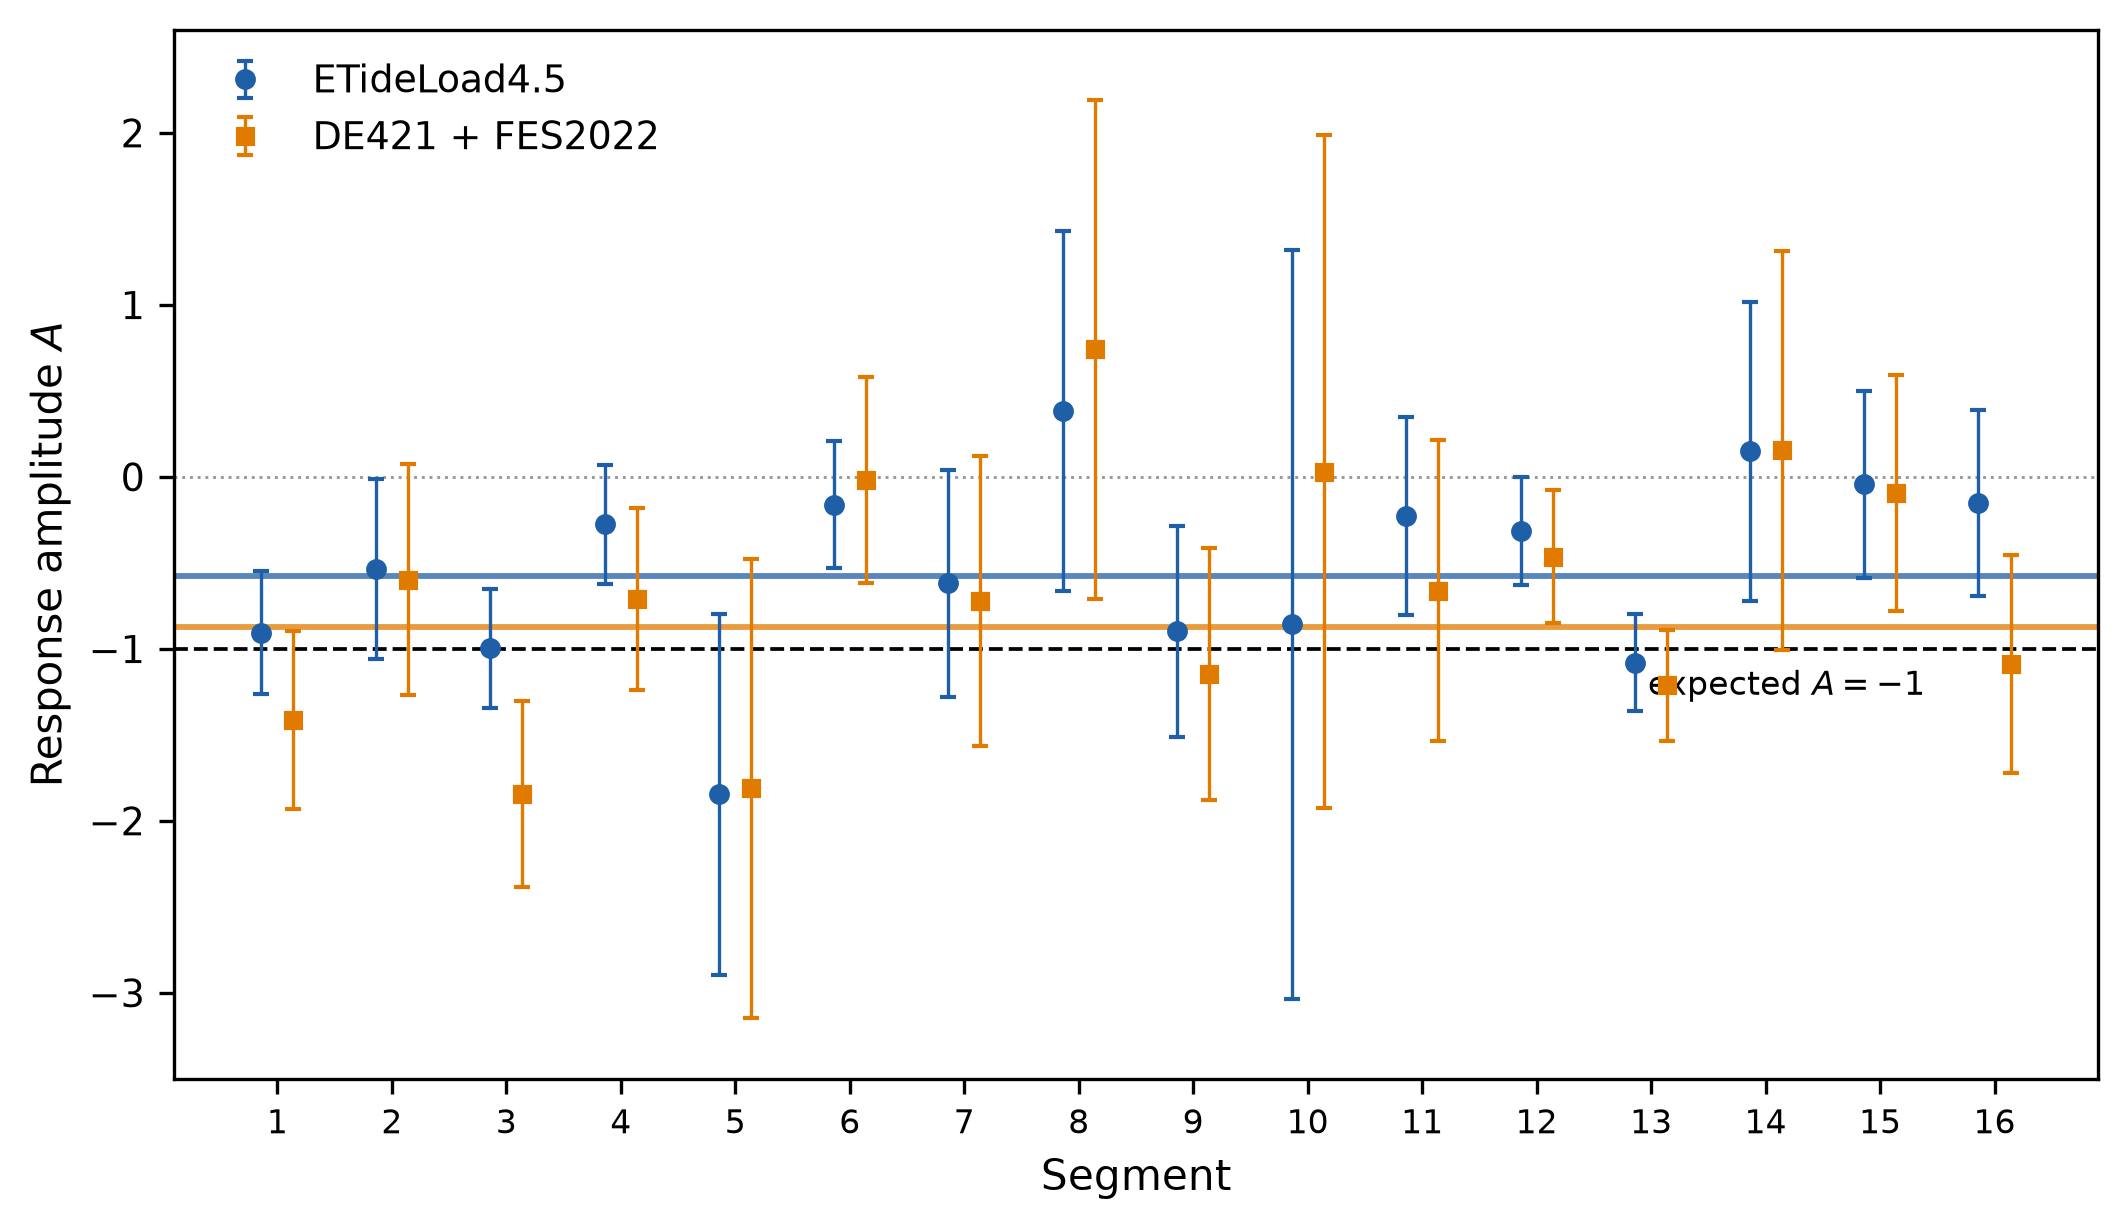
\includegraphics[width=\linewidth]{figs/fig4_tidal_response.png}
  \caption{Within-segment tidal correlation analysis.
  \textbf{(a)} Single-segment example: the 1200-s demeaned beat
  waveform (dots) and the tidal template scaled at the expected
  response $A=+1$ and at the fitted amplitude, for the ETideLoad4.5
  model. No single segment reaches a significant correlation on its
  own. \textbf{(b)} Per-segment response amplitudes $A$ for the two
  tide models, over the \nSeg~segments entering the ratio
  combination. Error bars are per-segment fit uncertainties from
  non-overlapping windows; the solid lines mark the precision-weighted
  combinations. In \tidalNegSeg~of the \nSeg~segments the correlation
  is positive for either model, and both precision-weighted amplitudes
  ($\tidalAmpOldE$ and $\tidalAmpNewE$) fall short of the expected
  response of $+1$ (dashed line), so the observed tidal coupling is
  smaller than any single template predicts.}
  \label{fig:tidal-response}
\end{figure}

\end{document}
